%!TEX root = ../main.tex

\par
After an Atlantic hurricane dissipates, the National Hurricane Center (NHC) determines the most accurate track of the storm, and collects various other information about the storm throughout its lifetime.
The data is available online as a comma-separated values file.
The available data includes information about the hurricane taken every six hours, from the formation of the storm to its dissipation.
This includes:
\begin{itemize}
	\item Latitude and longitude of the system center
	\item Landfall events
	\item Maximum sustained wind
	\item Minimum barometric pressure
	\item Maximum extent of hurricane and tropical storm winds
\end{itemize}

\par
The tracked latitude and longitude of the system center is one very important component of the dataset, as it allows us to examine the path a hurricane has taken throughout its lifetime.
It also implicity gives us information on where the hurricane formed, and can be used to compare different storms to see how similar they are.

\par
The maximum sustained wind and minimum batrometric pressure are another useful piece of information to track.
Both represent the peak strength of a hurricane at a given time, albeit in different ways.
Maximum sustained wind speed and minimum barometric pressure are direct measurements of the power of a storm.
In addition, the change in barometric pressure indicates whether a storm is strengthening or weakening.
% https://www.rhinobldg.com/understanding-barometric-pressure-in-hurricanes/

\par
Finally, tracking whether or not a hurricane made landfall, and the conditions when it made landfall, allows us to esimate how dangerous the hurricane was.
A strong hurricane which never makes landfall is much less hazardous than a weak hurricane that does.
This also allows us to make larger judgements as to the number of damaging hurricanes per year.

\begin{figure}
	\centering
	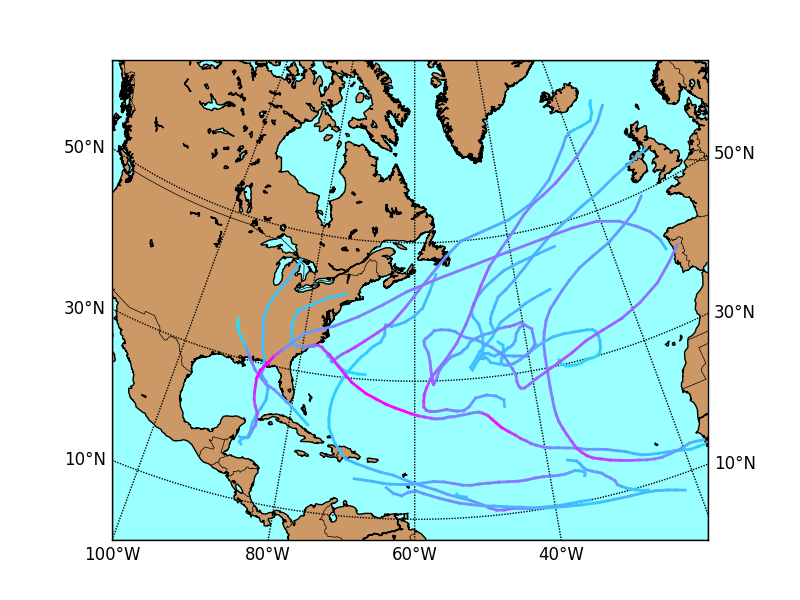
\includegraphics[width=\linewidth]{images/2018_max_winds.png}
	\caption{A map of the track of every Atlantic tropical storm in 2018. The color is scaled by the maximum wind speed.}
	\label{fig:2018_storm_tracks}
\end{figure}

\begin{figure}
	\centering
	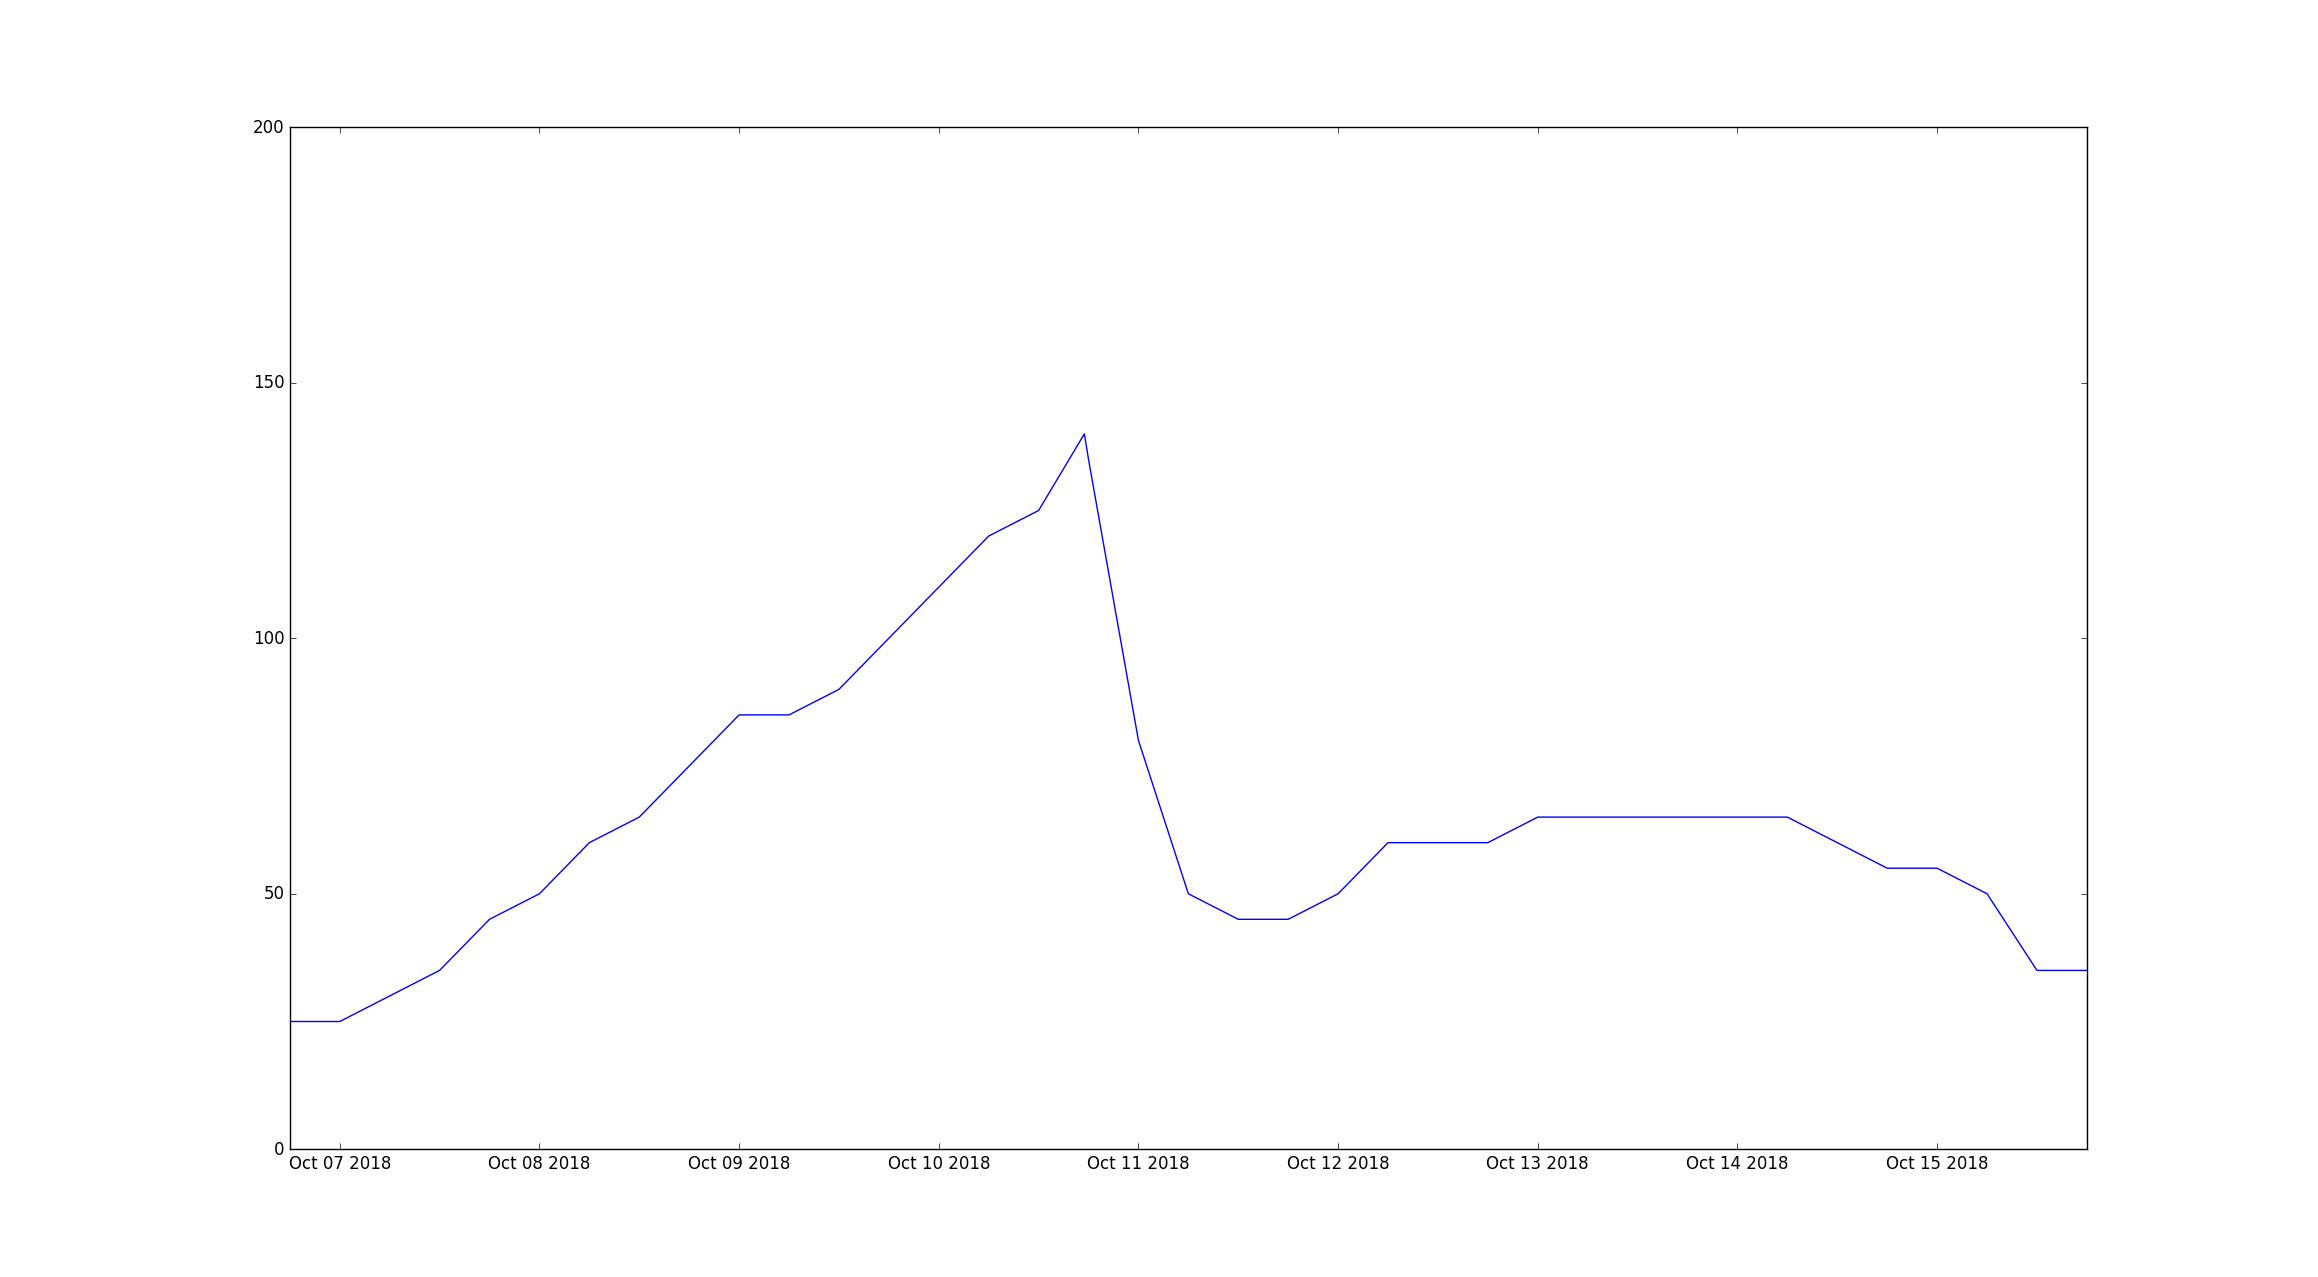
\includegraphics[width=\linewidth]{images/hurricane_michael_max_wind.png}
	\caption{A plot of the maximum wind speed of Hurricane Michael over its lifetime.}
\end{figure}